\documentclass[a4paper,11pt]{article}
\usepackage[T1]{fontenc}
\usepackage[utf8]{inputenc}
\usepackage{lmodern}
% \usepackage{hyperref} % fucking warnings
\usepackage{graphicx}
\usepackage{graphics}
\usepackage{rotating}
\usepackage{listings}
\usepackage{color}
\usepackage{listings}
\usepackage{amsthm}
\usepackage{amsmath}
\usepackage{amssymb}
\usepackage{algorithmic}
\usepackage{datatool}
\usepackage{caption}
\usepackage{subcaption}

% \newcommand{\encode}[1] {{ {}_{\llcorner}{#1}_{\lrcorner}}}

\title{Numerical Linear Algebra (CSE-6643) - Midterm take home exam}
\author{Arash Rouhani (rarash@gatech.edu) - gtid: 902951864}


\begin{document}

\maketitle

\section{Part I}

This task consists of (1) discretizing a differential equation into
linear equation, (2) solving the linear equation using own
written gauss elimination and (3) plotting,  timing and commenting on
results.

\subsection{Discretization}

For $n$ interior points we have $m=n+1$ interior slices. We define $h$
to $1/m$ which is the distance between the points. With this a natural
discretization appears

\[
  u''[i] = \frac{1}{2} - \frac{i}{m} = \frac{u[i+1]-2u[i]+u[i-1]}{h^2}
\]

Where $u$ is unknown, of course, we want to solve for it since it's a
differential equation. More precisely, $u[0]=u[m]=0$ are corresponding
to the given initial values and $u[i]$ exists for $i = 1..n$.

Now we want to form the typical equation $Ax=b$ such that solving for
$x$ gives all $u[i]$. The equation above gives us this scheme: Let $A$
be a tridiagonal matrix with only $-2$ in the diagonal and $1$ in its
sub- and super diagonal. Set $b_i$ to $(1/2-i*h)h^2$. $x_i$ is simply
$u[i]$ in this scheme.

\subsection{Solving a linear equation}

My implementation of gauss elimination is a direct source code
translation from the pseudo code from the book. I did not implement the
optimizations like not explicitly creating $P$ or let $A$ be overwritten
by $U$ or $L$. The $Ax=b$ is rewritten as $LUx=Pb=b'$, very much like
the discussion in the book (p. 152). As the book hints, I just use a
forward and backward elimination to solve the triangular systems. I
wrote both a forward and backward elimination, but they are not
attached.

\subsection{Results and analysis}

I did run it for the $n$s mentioned on the exam. I used matlabs
\texttt{tic toc} routines to time everything. Here are the results

\begin{lstlisting}
Elapsed time is 0.060627 seconds.    ( n = 50   )
Elapsed time is 0.238094 seconds.    ( n = 100  )
Elapsed time is 1.072788 seconds.    ( n = 200  )
Elapsed time is 5.368879 seconds.    ( n = 400  )
Elapsed time is 30.166895 seconds.   ( n = 800  )
Elapsed time is 194.438070 seconds.  ( n = 1600 )
Elapsed time is 1328.453620 seconds. ( n = 3200 )
\end{lstlisting}

We observe an increase in execution time by a factor between $6$ and
$7$. I would have guessed around $8$ because the $O(m^3)$ complexity
gets multiplied by $8$ when $m$ doubles.

\begin{figure}
        \begin{subfigure}[b]{1.0\textwidth}
          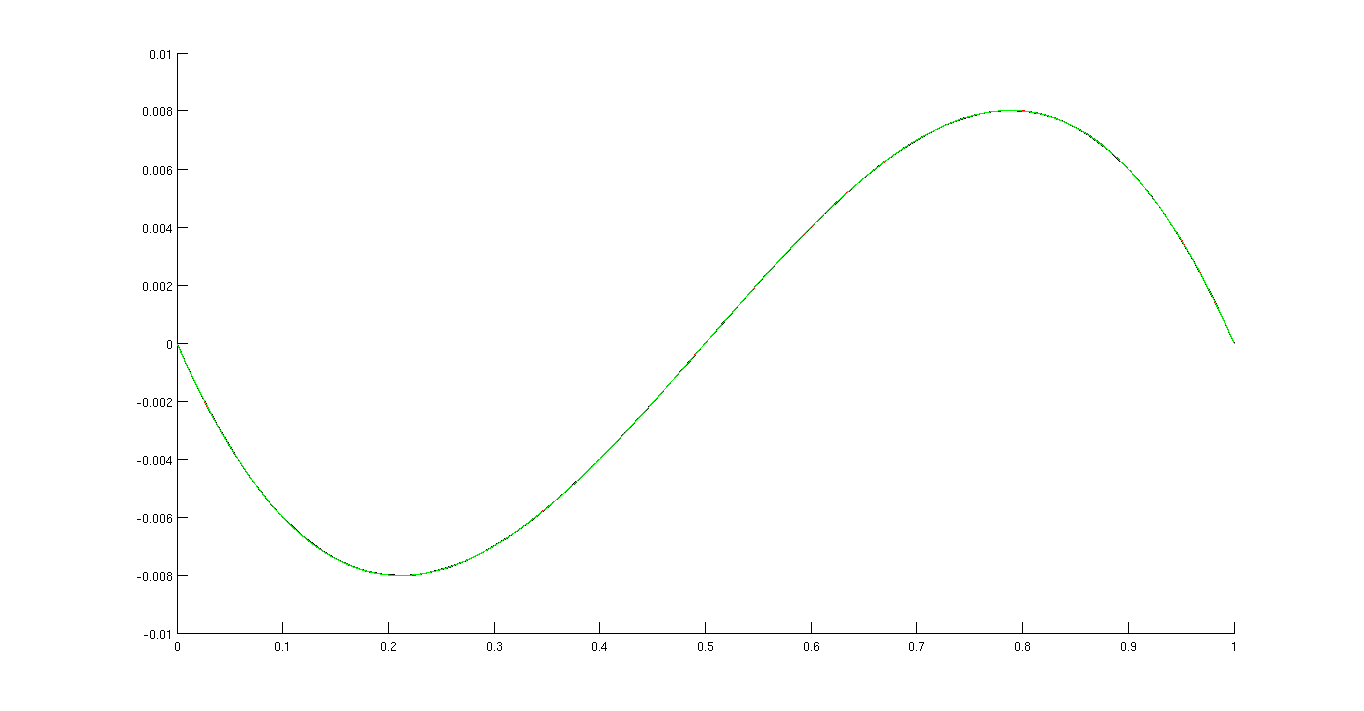
\includegraphics[width=\textwidth]{fig/all.png}
          \caption{The whole plot}\label{fig:wholeplot}
        \end{subfigure}

        \begin{subfigure}[b]{1.0\textwidth}
          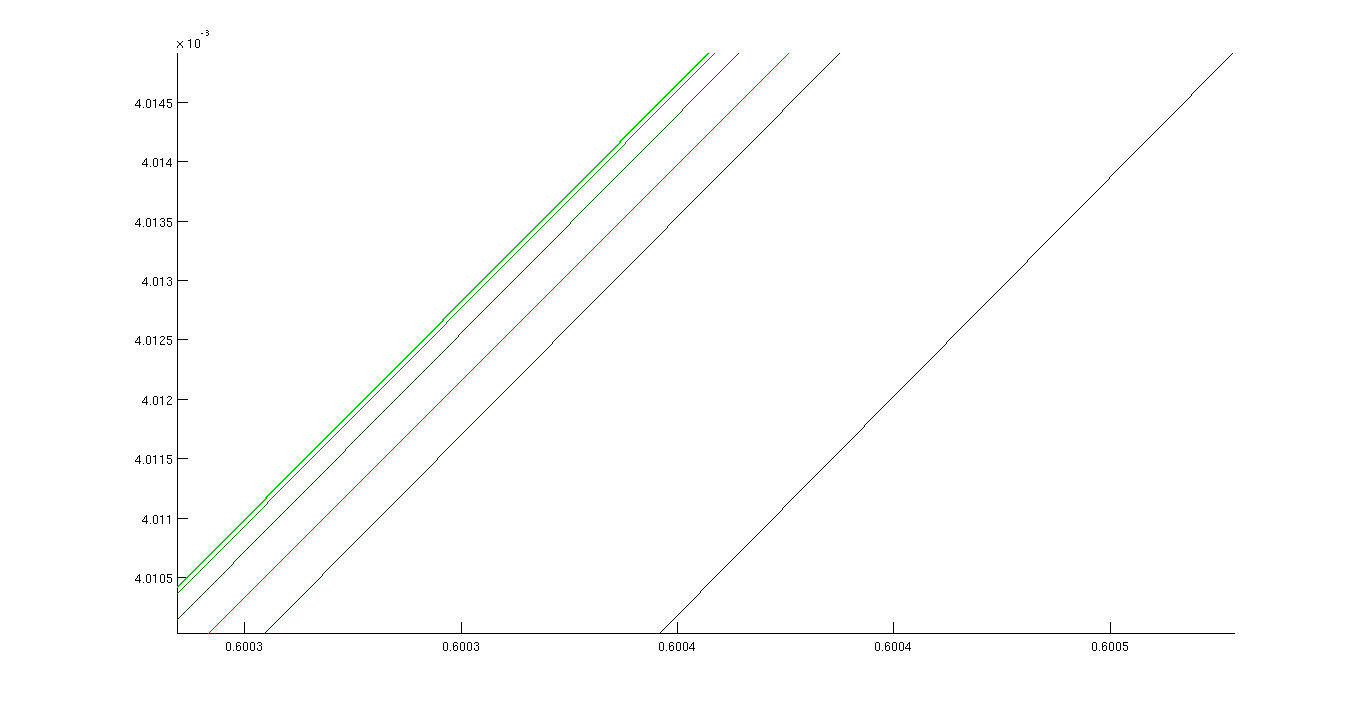
\includegraphics[width=\textwidth]{fig/azoom.png}
          \caption{One zooming}\label{fig:zooming}
        \end{subfigure}
        \caption{Plots of $u(x)$. The red line is the actual function.
        The others are estimations. The greener the line the higher
      $n$.}\label{fig:plots}
\end{figure}

I've included two plots, one which isn't zoomed and one which is highly
zoomed. The "actual function" in red is a symbolically expressed
function, the solution to the differential equation I solved by hand.

What I find surprising in the zoomed figure is that with a higher $n$
the green lines clearly are converging, but not towards the correct (red)
line.  This behavior persists even if I use matlab's "backslash" instead
of my Gaussian elimination. The difference is also much higher than the
machine epsilon, so it's not a stability issue. I'm not sure how
\texttt{fplot} works (which I plotted the red line with), but I believe
it might use a forward or backward difference scheme rather than the
centered difference scheme, that might explain why the estimation
doesn't converge to the actual value but to a value near it.

\subsubsection{Some extra experiments}

I also tried using matlabs in built \texttt{A\textbackslash b}. It's not until
$n>100000$ that matlab surpasses a second of execution time! Obviously
matlab can use the fact that the matrix is tridiagonal. Hence, matlab
confirms that using Gaussian elimination is very naive for this
particular problem since it'll not use the fact that $A$ is tridiagonal.

Another experiment I did was to profile my code, most of the execution
$>80\%$) time was spent on the line corresponding to the last line of
the gauss pseudo code from Algorithm 21.1 in the book.  Why? Because
it's the line making the algorithm $O(m^3)$ rather than $O(m^2)$.

\section{Part II}

\subsection{a}

Here is an algorithm to generate a matrix $A$ with the given singular values
$\Sigma$. Generate two random unitary matrices $U$ and $V$ and let $A = U
\Sigma V^*$. The way you generate the unitary matrices could be like this:

Let $P=I$ be a projector which is gonna make sure of the orthogonality of the
vectors we generate. For each $i=1 \dots n$, we first randomly create size $n$
row vector $a_i$. Now to ensure that it's orthogonal to all previous vectors,
we multiply it by $P$. To ensure that future vectors will be orthogonal to the
current vector we set $P$ to $P P_{\perp a_i}$. Also, after we have projected
$a_i$ we also normalize it. Hence each vector we create is orthogonal to all
previous ones and it's also of length 1 because it's normalized. Constructing
a matrix consisting of these $n$ vectors will be unitary.

In practice this algorithm is superfluous, because this is exactly
how the stable Gram Schmidt generates $Q$, only that the $a_i$ vectors isn't
random but based on the input, so we create our unitary matrices by feeding
random data to stable Gram Schmidt and only looking at it's $Q$ output.

\subsection{b and c}

My Gram Schmidt implementations are direct translations from the
pseudo code presented in the text book. So they are not interesting,
instead I decided to look at the results of the produced $Q$s and $R$s.

As for the householder transform, again I decided to translate the
pseudo code from the text book. However that only gives me $R$, to
produce $Q$ I use algorithm 10.3 from the book, which is
\emph{Implicit calculation of a Product $Qx$} where I set x = $I_i$ for
all $i = 1 \dots n$. The book recommend this way to explicitly construct
$Q$, which is why I choose this way.

The rest of this chapter will consist of \emph{Observations} and
\emph{Analysis}. The former will present various values I extracted from
$Q$ and $R$ for the three different factorizations. Indeed, some
observed values are notable and form interesting patterns meanwhile
others seem arbitrary. My analysis will explain why that's so.

\subsubsection{Observations}

I extract these values from the algorithms' $QR$ factorizations.

\begin{itemize}
  \item Look at the norms of the produced $Q$s. Ideally they should be $1$.
  \item The standard deviation for the values of $A-QR$. Ideally the
    standard deviations are $0$.
  \item Define two matrices $\Delta Q$ and $\Delta R$ to $Q_{classic} -
    Q_{stable}$ and $R_{classic} - R_{stable}$ respectively. Then plot both
    their row and column medians. For the medians of the upper
    triangular matrix $R$, I ignore the non upper values when
    calculating the median since they are always zero.

\end{itemize}

I choose to look at the norms and the standard deviations because they
are very familiar metrics easy to extract. As for the four different
medians, they might reveal patterns in how the entries will
become more and more subjected to instability as the algorithm
progresses, either column wise or row wise.

Let's first look at the data for $n=100$ and then see if
the pattern is particularly different for $n=150$.

\begin{table}[h]
  \begin{tabular}{r|c|c|c|}
    \multicolumn{1}{r}{}
     & \multicolumn{1}{c}{$Q_{classic}$ }
     & \multicolumn{1}{c}{$Q_{stable}$}
     & \multicolumn{1}{c}{$Q_{householder}$} \\
    \cline{2-4}
    $n=100$ & \input{data/norm-q-classi-100.dat}
            & \input{data/norm-q-stable-100.dat}
            & \input{data/norm-q-househ-100.dat}
            \\ \cline{2-4}
    $n=150$ & \input{data/norm-q-classi-150.dat}
            & \input{data/norm-q-stable-150.dat}
            & \input{data/norm-q-househ-150.dat}
            \\ \cline{2-4}
  \end{tabular}
  \caption{Norms for the different unitary $Q$ matrices}
  \label{tab:norms}
\end{table}

\begin{table}[h]
  \begin{tabular}{r|c|c|c|}
    \multicolumn{1}{r}{}
     & \multicolumn{1}{c}{$Q_{classic}$ }
     & \multicolumn{1}{c}{$Q_{stable}$}
     & \multicolumn{1}{c}{$Q_{householder}$} \\
    \cline{2-4}
    $n=100$ & \input{data/std-q-classi-100.dat}
            & \input{data/std-q-stable-100.dat}
            & \input{data/std-q-househ-100.dat}
            \\ \cline{2-4}
    $n=150$ & \input{data/std-q-classi-150.dat}
            & \input{data/std-q-stable-150.dat}
            & \input{data/std-q-househ-150.dat}
            \\ \cline{2-4}
  \end{tabular}
  \caption{The standard deviation for the values of $A-QR$}
  \label{tab:stds}
\end{table}

\newcommand{\genfig}[3] {{
    \begin{figure}
            \centering
            \begin{subfigure}[b]{1.0\textwidth}
                    \includegraphics[width=\textwidth]{fig/#1-#2-100}
                    \caption{$n = 100$}
            \end{subfigure}
            \begin{subfigure}[b]{1.0\textwidth}
                    \includegraphics[width=\textwidth]{fig/#1-#2-150}
                    \caption{$n = 150$}
            \end{subfigure}
            \caption{Medians of the columns of $\Delta #2$ #3}\label{fig:#1-#2}
    \end{figure}
  }}

\genfig{log-median-col}{Q}{logarithmized}
\genfig{median-row}{Q}{}
\genfig{log-median-col}{R}{logarithmized}
\genfig{log-median-row}{R}{logarithmized}

\subsubsection{Analysis}

There are clearly many interesting patterns here, but lets save the best
for the last.

\textbf{Table \ref{tab:stds} has no outlier}. The standard deviations
are all very small and about the same size. Why? Because the algorithms
we use are at worst only instable and the small singular values (part of
input) will only provoke errors of the size of the machine error. The
algorithms are however not incorrect. They successfully compute a $QR$
factorization.  Put simply, the standard deviation would have only been
big if the algorithm itself were completely incorrect, the ones we use
are only unstable and thus we only get a very small error.

\textbf{There is no pattern in figure \ref{fig:median-row-Q}}. Well, Both
Gram Schmidt algorithms are iteratively constructing $Q$ in the sense
that it's built column vector by column vector. So when looking at a row,
it will consist values from the columns created at all the different
steps of the iteration. So the diffused set of values will not yield any
pattern when scanning along the rows.

\textbf{Table \ref{tab:norms}}. It's clear what happens with the norm
for $Q_{stable}$ and $Q_{householder}$. The former converges to $\sqrt{2}$
and the latter stays at exactly $1$. For the classic algorithm it
doesn't seem to diverge but it's still increasing significantly when
increasing $n$ from $100$ to $150$.

\textbf{Figure \ref{fig:log-median-col-Q}, \ref{fig:log-median-col-R},
\ref{fig:log-median-row-R} are linear then flattens}. The
"column median figures" (\ref{fig:log-median-col-Q} and
\ref{fig:log-median-col-R}) clearly flattens at around $i=25$
independent of $n$. Similarly in figure \ref{fig:log-median-row-R}, the
median of the rows of $R$, a flattening is happening at $i=50$. Of
course there is no purely mathematical significance with the number $50$
nor $25$, so I suspected that my machine's simplification of the real
numbers, the floats, was the culprit. Indeed matlab reported that
the machine epsilon is $2^{-52}$ when typing \texttt{help eps}.


\end{document}
